\documentclass[conference]{IEEEtran}
\renewcommand\IEEEkeywordsname{Keywords}
\usepackage{natbib}
\usepackage{amsmath}
\usepackage{graphicx}
\usepackage{float}


\usepackage{caption}
\captionsetup{labelsep=space,justification=justified,singlelinecheck=off}
% correct bad hyphenation here
\hyphenation{op-tical net-works semi-conduc-tor}


\begin{document}

\title{Combination Normal Sparse and Discriminative Deep Belief Networks}

\author{\IEEEauthorblockN{Faisal Khalid}
\IEEEauthorblockA{Department of Computer Science\\
University of Indonesia\\
Depok, West Java, Indonesia\\
faisal.khalid.si@gmail.com}
\and

\IEEEauthorblockN{Mohamad Ivan Fanany}
\IEEEauthorblockA{Department of Computer Science\\
University of Indonesia\\
Depok, West Java, Indonesia\\
ivan@cs.ui.ac.id}}

% make the title area
\maketitle

% As a general rule, do not put math, special symbols or citations
% in the abstract
\begin{abstract}
Sparse representations are better than non-sparse in efficiency. This paper
aim to find the best structure of combination sparsity and
discriminative DBN. We use DBN architecture with 784 as input,
500 hidden unit, 500 hidden unit, 2000 hidden unit, and 10 as
output. We took 3 step in this experiment, preliminary,
intermediate and the final result. Every analysis of each step is a
background to the next step. We use normal sparse for sparse
generative and sparse discriminative. Experimental studies on
MNIST dataset shows that the best structure in combination
normal sparse and discriminative deep belief networks are with
input- generative (Contrastive Divergence) - generative
(Contractive Divergence) – normal sparse
discriminative
(Contractive Divergence).
\end{abstract}

\begin{IEEEkeywords}
Restricted Boltzmann Machines, Normal Sparse , Discriminative Deep Belief Network, Deep Belief Networks
\end{IEEEkeywords}
% no keywords

\IEEEpeerreviewmaketitle



\section{Introduction}
For some theoretical reason, deep architecture was
suggested \cite{keyvanrad1}.
DBN (Deep Belief Network) is a good tool which can solve local minima and time-consuming problem in deep models.DBN can create a neural
networks which have several hidden layers \cite{liu1}.
Computing connection between the hidden layer and visible
layer in DBN is so difficult. Gibbs sampling can be used,
although it takes a long time. So it is impossible to
do.Contrastive Divergence (CD)\cite{carreiraperpinan1}, PCD \cite{tieleman1}, and FEPCD \cite{keyvanrad2}
are used to solved that problem.
Feature extraction was an interest in recently. One of the novel research in feature extraction is deep learning with sparse coding\cite{olshausen1}. Sparsity is a key in Deep Belief Networks to make optimization. Bengio argued that in fixed size representations, sparse in better than non-sparse representation \cite{bengio1}.
Several previous studies have done in sparse and
discriminative deep belief network. The studies in\cite{tieleman1}
proposed semi-supervise learning by using discriminative
Deep Belief Network(DDBN). In written digit competition ( ICDAR 2013), sparse deep
belief networks and denoising autoencoder to a new dataset has been proposed \cite{walid1}.\cite{larochelle1} using discriminative RBM as classifiers can
improve performance in a semi-supervised learning. The
studies in\cite{halkias1} present a theoretical approach for sparse
constraints in the DBN.
DB=BN is created by stacking RBMs, therefore the improvement in RBMs are due to the improvement of DBN. We argue that combination sparsity and discriminative
DBN will increase the accuracy, but no one ever proposed
what structure of that combination will give the best accuracy .
This paper aim to find the best structure of combination
sparsity and discriminative DBN. For ease of reproduction of
results, this paper is performed on publicly available dataset
(MNIST Dataset). This paper organized as follows. Section II
explain literature study. Section III describes proposed
methods. Section IV describe the experimental setup. Section
V explain the experimental result and discussions. Finally,
conclusions are given in section VI.

\section{Literature Review}
\subsection{Restricted Boltzmann Machines (RBM)}
Restricted Boltzmann Machines (RBM) is a generative model of which had been
use in various fields, such as the images processing, speech, bags of word, and motion capture [19]. RBM consists of two layers, namely, visible layer and the hidden layer. In RBM are connected only
visible throughout the entire unit with hidden units, but there is no connection
between visible units or between hidden units.
Joint configuration between visible and hidden (v, h) can be formulated as follows:
\begin{equation} 
E(v,h)=-\sum_{i \epsilon visible }a_{i}v_{j} -\sum_{j \epsilon hidden} b_{j}h_{j} - \sum{v_{i}h_{j}w_{ij}}
\end{equation}

Where $v_{i} h_{j}$ is a state of visible unit $i$, $j$ hidden unit, and $a_{i}, b_{j}$ is
bias, and $w_{ij}$ is a unit of weight between the visible and the hidden unit $i j$. probability
of each pair of visible and hidden can be calculated using the energy function:
\begin{equation}
p(v,h)=\frac{1}{Z}^{-E(v,h)}
\end{equation}

Z is the partition function, which is the sum of all probabilitas of each pair of visible units and hidden units.
\begin{equation}
Z= \sum_{v,h}e^{-E(v,h)}
\end{equation}

The probability of RBM, could be improved by fine-tuning parameters. The lower the energy the greater the probability and vice versa. The probability of visible units of all i can be calculated to be 1 by the following equation:
\begin{equation}
p(v_{i}=1|h)=\sigma (a_{i}+\sum_{j}h_{i}w_{ij})
\end{equation}

Where $\sigma $ is the sigmoid function, 1 / (1 + exp (-x)).  Probability of a hidden unit $j$ to be 1 can be calculated by the equation:
\begin{equation}
p(h_{j}=1|v)=\sigma (b_{j}+\sum_{i}v_{j}w_{ij})
\end{equation}
\subsection{Normal Sparse RBM}
The goal of sparsity in RBM is to fire up or force activation probability of hidden units to zero using some regulation term.  Normal sparse using a variance parameter and normal
function properties as regulation term\cite{keyvanrad1}. The degree of sparseness can be controlled by variance. 
Sparse RBM can learn by using this step\cite{lee1}
\begin{enumerate}
	\item Use an approximation to the
	gradient of log likelihood to update the parameters.
	\item Adding regulation term to update the parameter.
	\item Repeat steps 1 and 2 until convergence.
\end{enumerate}

The different regulation term with different behavior has been proposed 
in \cite{keyvanrad1}. The regulation term  was they used are variance and normal probability
density function.
\begin{equation}\label{eq:1}
L_{sparsity}=\sum_{j=1}^{n}f(q_{j},p,\sigma^{2})
\end{equation}
According to \ref{eq:1} the gradient if regularization
term must be used in step 2. The gradient of regularization
term can be computed as follows :
\begin{multline}
\frac{\partial}{\partial b_{j}}L_{sparsity }\oe  \frac{1}{m}\left ( p-\frac{1}{m}\sum_{l=1}^{m}q_{j}^{(l)} \right )f\left ( q_{j},p,\sigma^{2}   \right )\\ \times\sum_{l=1}^{m}q_{j}^{(l)}\left ( 1-q_{j}^{(l)} \right )
\end{multline}

\subsection{Discriminative Restricted Boltzmann Machines (DRBM)}
The important thing in classification is to have a good and
correct classification. we can optimize directly 
$ p\left ( x|y \right )$  below\cite{larochelle1}
\begin{equation}
L_{disc}\left ( D_{train} \right )= -\sum_{i=1}^{\left | D_{train} \right |}log    p\left ( y_{i}|x_{i} \right )
\end{equation}
Based on $L_{disc}$, discriminative RBM (DRBM) can refer to
RBMs trained. Contrastive divergence can be used in DRBM
to training\cite{taylor1}. Gradient can be computed as:
\begin{multline}
\frac{\partial log p\left ( y_{i}|x_{i} \right )}{\partial\theta } =\sum_{j}sigm\left ( o_{yj}\left ( x_{i} \right ) \right )\frac{\partial o_{yj}\left ( x_{i} \right )}{\partial\theta}
\\ -\sum_{i,y^{*}}sigm\left ( o_{y^{*}}\left ( x_{i} \right ) \right )p\left ( y^{*}|x_{i} \right )\frac{\partial o_{yj}\left ( x_{i} \right )}{\partial\theta}
\end{multline}

Where $o_{yj}\left ( x \right )=c_{j}+\sum_{k}W_{jkxk} + U_{jy}$. Stochastic gradient descent
optimization can be done by computed this gradient with
efficient. Fine-tuning the top RBM of DBN is using this
approach\cite{hinton1}.
\subsection{Free Energy in Persistent Contrastive Divergence}
Gibbs sampling is an appropriate method as in RBM
because each unit in RBM is independent of other units.
CD, PCD, or FEPCD\cite{keyvanrad2} can be used to obtain proper
samples from the model because impossible to use Gibbs
sampling.
In PCD methods, many persistent chains can be run in
parallel. If we can define the criteria for a good chain, and for
computing the gradient sample would be more accurate.
Defining the best chain by using the free energy is as
follows \cite{hinton2} :
\begin{multline}
F\left ( v \right )=-\sum_{i}v_{i}a_{i}-\sum_{j}q_{j}I_{j}+
\\ \sum_{j}\left ( q_{j}log q_{j}+\left ( 1-q_{j} \right )log\left ( 1-q_{j} \right ) \right )
\end{multline}

Sum of input to hidden unit $j$ is equal with $I_{j}=b_{j}+\sum v_{i}w_{ij}$
and $q_{j}=q(I_{j})$ is equal to activation probability of hidden unit
$h_{j}$ given $v$ and $q$ is logistic function. An equivalent and
simpler equation for computing $F(v)$ is as follows:
\begin{equation}
F(v)=-\sum_{i}v_{i}a_{i}-\sum_{j}log(1+e^{I_{j}})
\end{equation}
\section{Proposed Method}
Fig. 1. Show proposed method in this paper. The proposed
method including three steps as follows
\begin{enumerate}
	\item Train the first RBM by inputting the original data and
	fixing up the parameters of this RBM. Then we use
	these output as the input of the second RBM and the
	rest can be done in the same manner.
	\item We use modified the RBM with normal sparse.
	\item Fine-tuning: using Back Propagation (BP). We use
	gradient-descent algorithm to revise the weight
	matrix of the whole network.
	
\end{enumerate}

\begin{figure}[h]
	\centering
	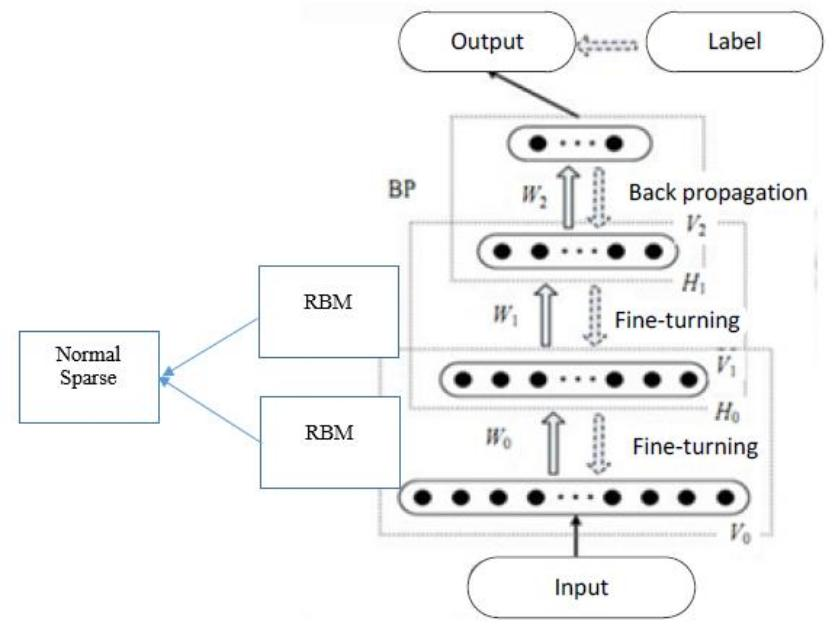
\includegraphics[width=.25\textwidth]{pics/proposedMethod.jpg}
	\caption{Proposed Method}
	\label{fig1}
\end{figure}

\section{Experimental Setup}
The experimental study is carried out by used DeeBNet
Matlab toolbox\cite{keyvanrad3}. 
We use DBN architecture with 784 as input, 500 hidden
unit, 500 hidden unit, 2000 hidden unit, and 10 as output. This
architecture we used in each experiment.
\subsection{Data}
The small MNIST and MNIST dataset were used to evaluate the different DBN models. MNIST dataset includes images of handwritten digits\cite{lecun}. The dataset was divided to train and
test part including 60,000 and 10,000 images respectively. For preliminary and intermediate we use small MNIST. Small MNIST is part of MNIST dataset but only 6000 training data and 1000 testing data.
\section{Experiment Result And Analysis}
This section described the performance of DBN by
comparing with other modified DBN. We took 3 step in this
experiment, preliminary, intermediate and final result. Every
analysis of each step is a background to the next step. We use
normal sparse for sparse generative and sparse discriminative.
\subsection{Preliminary Result}
In this step, we combine generative RBM, normal sparse
generative RBM, discriminative RBM, and normal sparse
generative RBM to find the best architecture to obtain best
accuracy. Table \ref{preRes} shown the accuracy obtained. Fig \ref{fig2} sparsity feature for 2$^{nd}$ Fig \ref{fig3} sparsity feature for 4$^{th}$ experiment. Fig \ref{fig4} Shown reconstruction for 1$^{st}$ experiment. Fig \ref{fig5} reconstruction for
4$^{th}$ experiment.

\begin{table}[h]
		\caption{Accuracy Obtained In Preliminary Result}
	\centering

	\label{preRes}
	\begin{tabular}{|l|l|c|c|c|c|}
		\hline
		\multicolumn{1}{|c|}{\textbf{\begin{tabular}[c]{@{}c@{}}Exp.\\ No\end{tabular}}} & \multicolumn{1}{c|}{\textbf{DBN Structure}} & \textbf{\begin{tabular}[c]{@{}c@{}}Error\\ Before\\ BP\end{tabular}} & \textbf{\begin{tabular}[c]{@{}c@{}}Error\\ After\\ BP\end{tabular}} & \textbf{\begin{tabular}[c]{@{}c@{}}Accuracy\\ (\%)\end{tabular}} & \textbf{Epoch} \\ \hline
		1                                                                                & Input- SG-SG-SD                             & 0.568                                                                & 0.055                                                               & 99.945                                                           & 200            \\ \hline
		2                                                                                & Input-G-G-D                                 & 0.063                                                                & 0.044                                                               & 99.956                                                           & 175            \\ \hline
		3                                                                                & Input-SG-SG-D                               & 0.063                                                                & 0.095                                                               & 99.905                                                           & 200            \\ \hline
		4                                                                                & Input-G-G-SD                                & 0.067                                                                & 0.038                                                               & 99.962                                                           & 124            \\ \hline
		5                                                                                & Input-SG-G-SD                               & 0.31                                                                 & 0.045                                                               & 99.955                                                           & 200            \\ \hline
		6                                                                                & Input-G-SG-D                                & 0.115                                                                & 0.048                                                               & 99.952                                                           & 200            \\ \hline
	\end{tabular}
\end{table}

SG  : Normal Sparse Generative RBM
\\G : Generative RBM
\\SD : Sparse Discriminative RBM
\\D: Discriminative RBM
\begin{figure}[h]
	\centering
	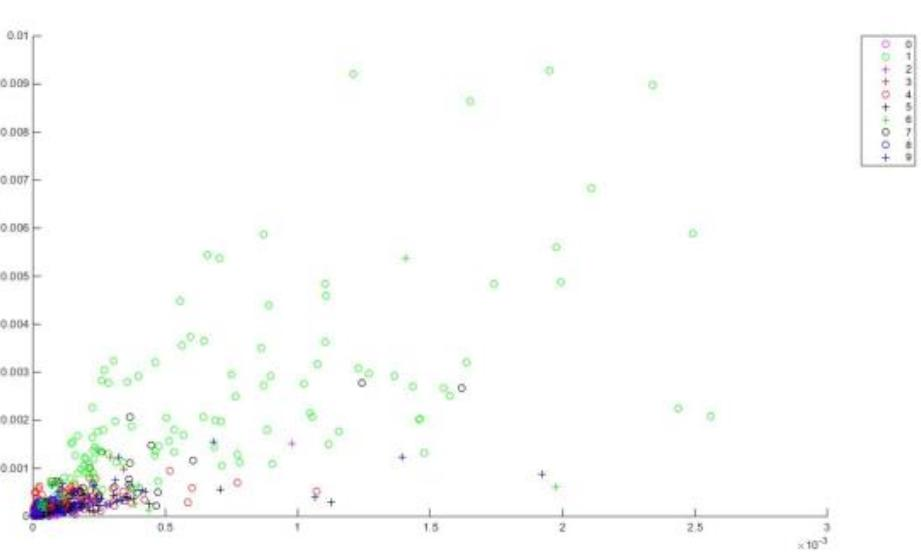
\includegraphics[width=.25\textwidth]{pics/fig2.jpg}
	\caption{Sparsity feature 2$^{nd}$ experiment}
	\label{fig2}
\end{figure}

\begin{figure}[h]
	\centering
	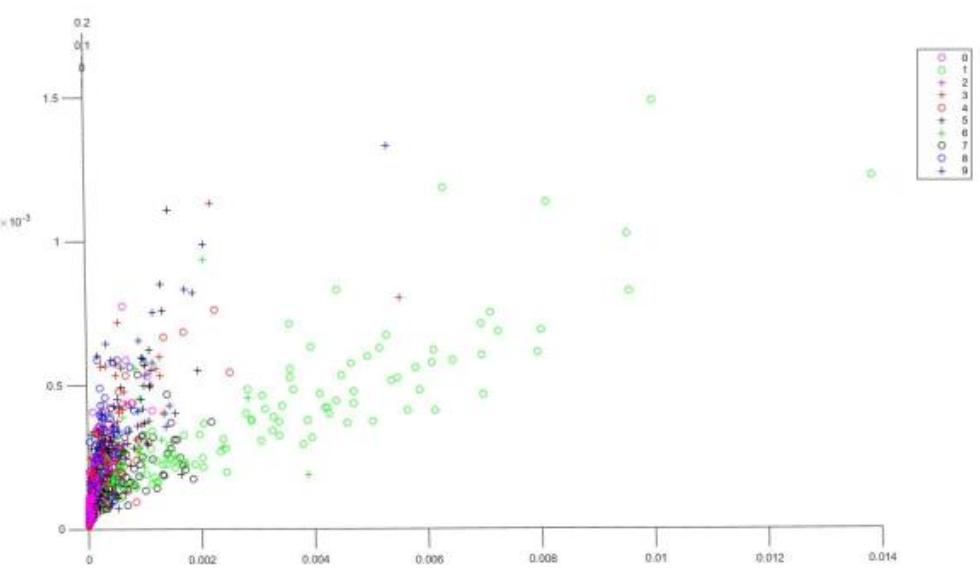
\includegraphics[width=.25\textwidth]{pics/fig3.jpg}
	\caption{Sparsity feature 4$^{th}$ experiment}
	\label{fig3}
\end{figure}

\begin{figure}[h]
	\centering
	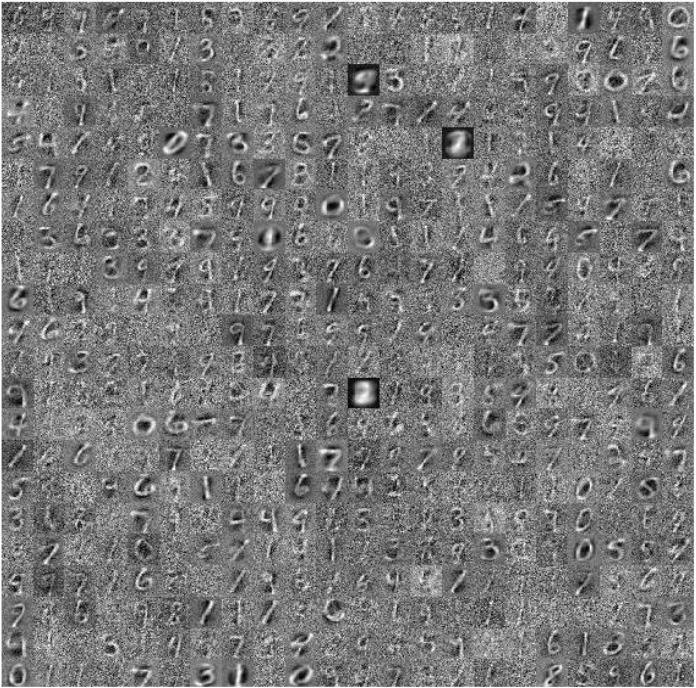
\includegraphics[width=.25\textwidth]{pics/fig4.jpg}
	\caption{RBM hidden layer in 1$^{st}$ experiment}
	\label{fig4}
\end{figure}

\begin{figure}[h]
	\centering
	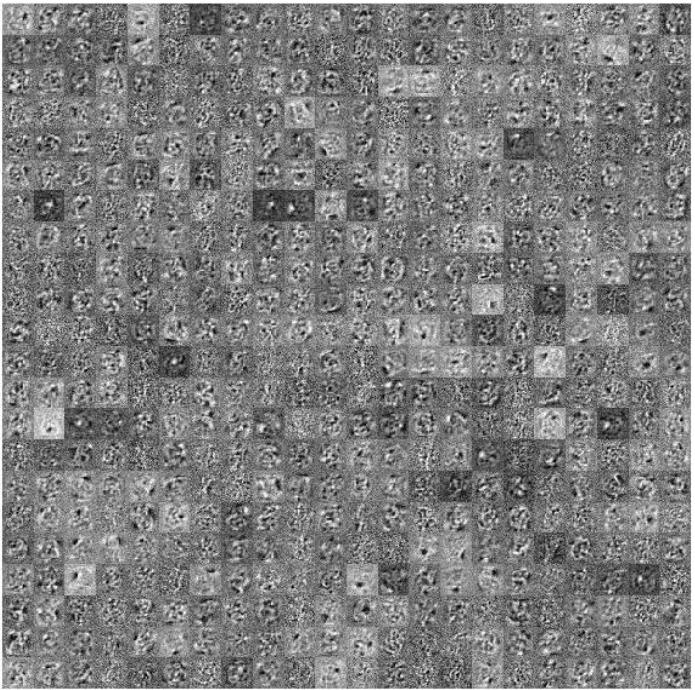
\includegraphics[width=.25\textwidth]{pics/fig5.jpg}
	\caption{RBM hidden layer in 4$^{th}$ experiment}
	\label{fig5}
\end{figure}

From  table \ref{preRes}, we obtained 99.96.2% as the best accuracy
with 124 epoch. Accuracy obtained using input-generative-
generative-Sparse Discriminative. Based on fig \ref{fig2} and fig \ref{fig3},
a sparse feature can obtain by using sparse distributive RBM.
Fig \ref{fig4} and fig \ref{fig5} shown that from reconstruct, generative RBM
make the feature more general than sparse generative RBM.

\subsection{Intermediate Result}
Based on preliminary result, we know that the best result is
using input-generative-generative-Sparse Discriminative with
99.962% accuracy and 124 epoch. In intermediate experiment,
we do experiment with another likelihood method, named
FEPCD. In this experiment, we implement FEPCD in our DBN
structure and compare with CD. The experiment result shown in
table II. Fig \ref{fig6},\ref{fig7},\ref{fig8},\ref{fig9} shown that the confusion matrix for each
experiment.
\begin{table}[h]
	\centering
	\caption{Accuracy Obtained In Intermediate Result}
	\label{interRes}
	\begin{tabular}{|l|l|l|l|l|}
		\hline
		\multicolumn{1}{|c|}{\textbf{\begin{tabular}[c]{@{}c@{}}Exp.\\ No\end{tabular}}} & \multicolumn{1}{c|}{\textbf{DBN Structure}}                                  & \multicolumn{1}{c|}{\textbf{\begin{tabular}[c]{@{}c@{}}Error\\ Before\\ BP\end{tabular}}} & \multicolumn{1}{c|}{\textbf{\begin{tabular}[c]{@{}c@{}}Acc\\ (\%)\end{tabular}}} & \multicolumn{1}{c|}{\textbf{Epoch}} \\ \hline
		1                                                                                & Input- G(CD)-G(CD)-SD(CD)                                                    & 0.0850                                                                                    & 99.8                                                                                  & 154                                 \\ \hline
		2                                                                                & \begin{tabular}[c]{@{}l@{}}Input-G(FEPCD)-G(FEPCD)\\ -SD(FEPCD)\end{tabular} & 0.1000                                                                                    & 99.9                                                                                  & 200                                 \\ \hline
		3                                                                                & Input- G(CD)-G(CD)-SD(FEPCD)                                                 & 0.0890                                                                                    & 99.8                                                                                  & 116                                 \\ \hline
		4                                                                                & \begin{tabular}[c]{@{}l@{}}Input- G(FEPCD)-G(FEPCD)\\ -SD(CD)\end{tabular}   & 0.1090                                                                                    & 99.8                                                                                  & 125                                 \\ \hline
	\end{tabular}
\end{table}

\begin{figure}[h]
	\centering
	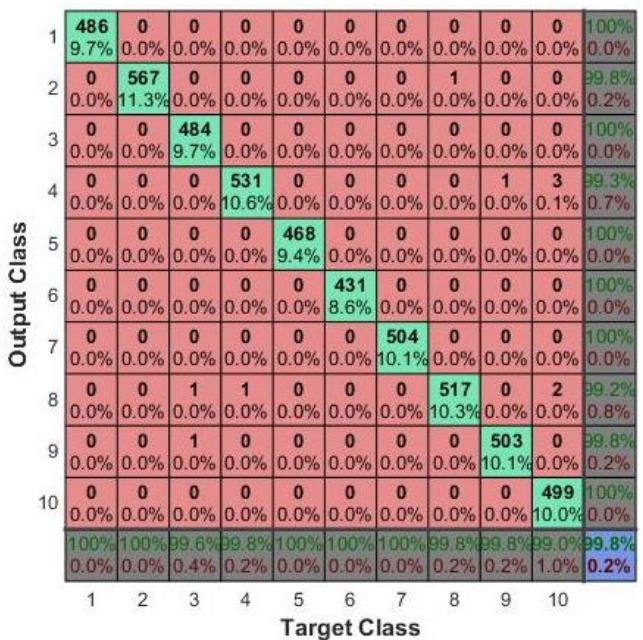
\includegraphics[width=.25\textwidth]{pics/fig6.jpg}
	\caption{1$^{st}$ intermediate experiment confusion matrix}
	\label{fig6}
\end{figure}

\begin{figure}[H]
	\centering
	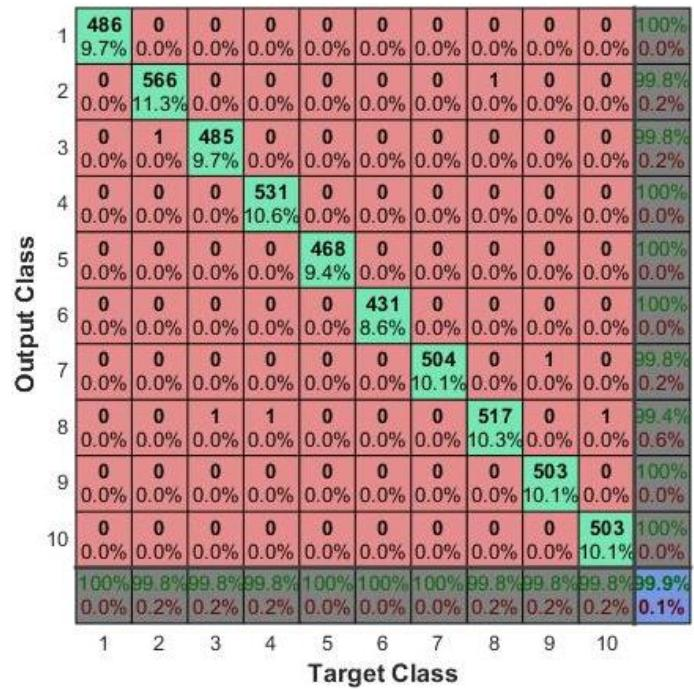
\includegraphics[width=.25\textwidth]{pics/fig7.jpg}
	\caption{2$^{nd}$ intermediate experiment confusion matrix}
	\label{fig7}
\end{figure}

\begin{figure}[H]
	\centering
	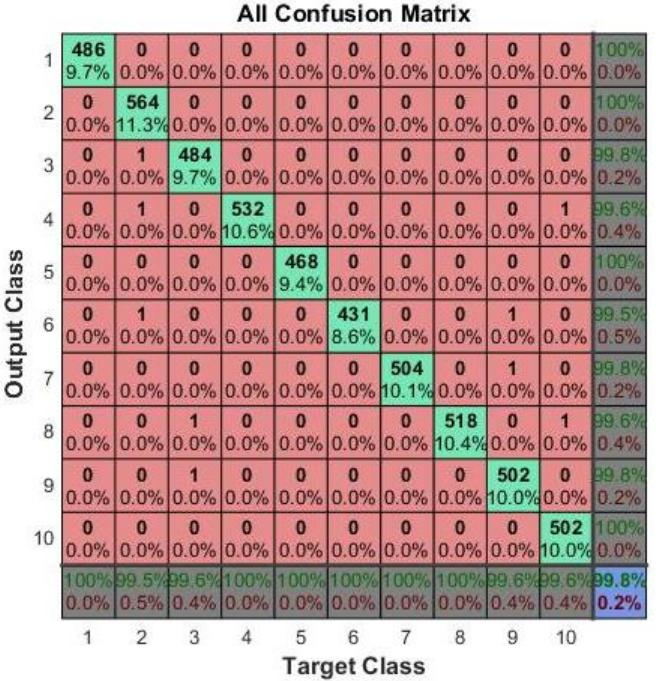
\includegraphics[width=.25\textwidth]{pics/fig8.jpg}
	\caption{3$^{rd}$ intermediate experiment confusion matrix}
	\label{fig8}
\end{figure}

\begin{figure}[H]
	\centering
	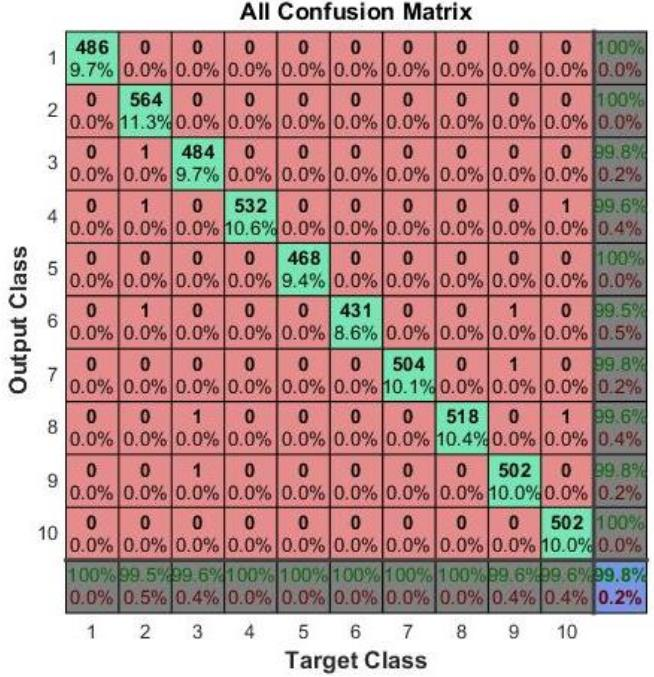
\includegraphics[width=.25\textwidth]{pics/fig9.jpg}
	\caption{4$^{th}$ intermediate experiment confusion matrix}
	\label{fig9}
\end{figure}

From all experiments, we got conclusion that best accuracy obtained is 99.8% with input- generative (FEPCD)-
generative (FEPCD)-sparse generative (FEPCD) and 116
epoch.
\subsection{Final Result}
From intermediate result, we got conclusion that used
FEPCD in all of RBM is better that CD, but time-consuming. For final result we did experiment for:
\begin{itemize}
	\item Input- Generative(CD) - Generative(CD) - Sparse
	Generative(CD)
	\item Input-Generative(CD)-Generative(CD)-Sparse
	Generative(FEPCD)
\end{itemize}

We choose Input - Generative(CD) - Generative(CD) -
Sparse Generative (FEPCD) because based on the intermediate result, this structure gives good accuracy and smallest epoch.
The experiment results shown in table \ref{finRes}. Confusion matrix
for all experiment shown in fig \ref{fig10} and fig \ref{fig11}. For final
experiment, we use full MNIST dataset.
\begin{table}[H]
	\centering
	\caption{Accuracy Obtained In Final Result}
	\label{finRes}
	\begin{tabular}{|l|l|l|l|l|}
		\hline
		\multicolumn{1}{|c|}{\textbf{\begin{tabular}[c]{@{}c@{}}Exp.\\ No\end{tabular}}} & \multicolumn{1}{c|}{\textbf{DBN Structure}}                                  & \multicolumn{1}{c|}{\textbf{\begin{tabular}[c]{@{}c@{}}Error\\ Before\\ BP\end{tabular}}} & \multicolumn{1}{c|}{\textbf{\begin{tabular}[c]{@{}c@{}}Acc\\ (\%)\end{tabular}}} & \multicolumn{1}{c|}{\textbf{Epoch}} \\ \hline
		1                                                                                & Input- G(CD)-G(CD)-SD(CD)                                                    & 0.0850                                                                                    & 99.8                                                                                  & 154                                 \\ \hline
		2                                                                                & \begin{tabular}[c]{@{}l@{}}Input-G(FEPCD)-G(FEPCD)\\ -SD(FEPCD)\end{tabular} & 0.1000                                                                                    & 99.9                                                                                  & 200                                 \\ \hline
		3                                                                                & Input- G(CD)-G(CD)-SD(FEPCD)                                                 & 0.0890                                                                                    & 99.8                                                                                  & 116                                 \\ \hline
		4                                                                                & \begin{tabular}[c]{@{}l@{}}Input- G(FEPCD)-G(FEPCD)\\ -SD(CD)\end{tabular}   & 0.1090                                                                                    & 99.8                                                                                  & 125                                 \\ \hline
	\end{tabular}
\end{table}

\begin{figure}[H]
	\centering
	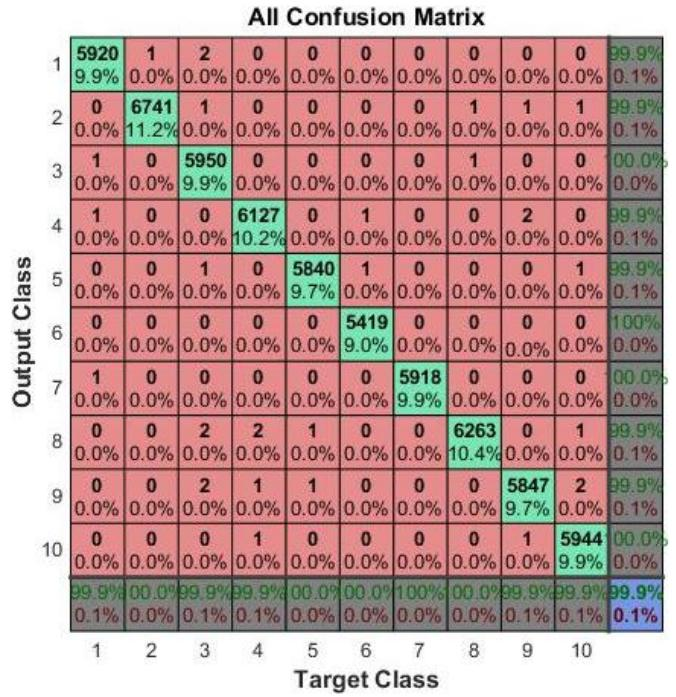
\includegraphics[width=.25\textwidth]{pics/fig10.jpg}
	\caption{1$^{st}$ final experiment confusion matrix}
	\label{fig10}
\end{figure}

\begin{figure}[H]
	\centering
	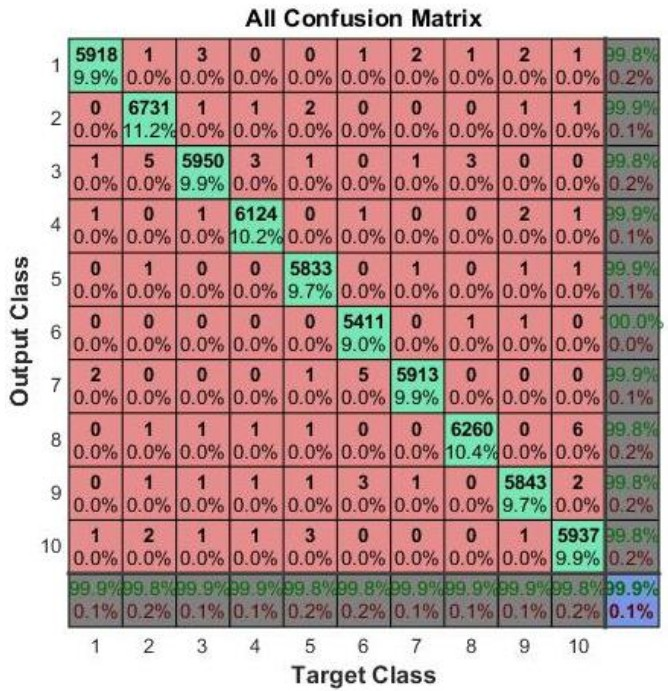
\includegraphics[width=.25\textwidth]{pics/fig11.jpg}
	\caption{2$^{nd}$ final experiment confusion matrix}
	\label{fig11}
\end{figure}


\section{Conclusion}
This paper investigates the best structure in combination
normal sparse and discriminative deep belief network. Our
experimental result shows that DBN with input- generative
(Contrastive Divergence) - generative (Contractive
Divergence) – normal sparse discriminative (Contractive
Divergence) give the best accuracy. It is obtained 99.9862%.
Sparse Discriminative make the sparse feature. Sparse feature
give better accuracy that nonsparse feature.


% use section* for acknowledgment
\section*{Acknowledgment}


The authors would like to thank...

\bibliographystyle{unsrt}
\bibliography{pustaka}






% that's all folks
\end{document}


